\documentclass[10pt,twocolumn,letterpaper]{article}

\usepackage{cvpr}
\usepackage{times}
\usepackage{epsfig}
\usepackage{graphicx}
\usepackage{amsmath}
\usepackage{amssymb}
\usepackage{bm}
\usepackage{algorithm}
\usepackage[noend]{algpseudocode}
\usepackage{algorithmicx}
% Include other packages here, before hyperref.

% If you comment hyperref and then uncomment it, you should delete
% egpaper.aux before re-running latex.  (Or just hit 'q' on the first latex
% run, let it finish, and you should be clear).
\usepackage[breaklinks=true,bookmarks=false,colorlinks,linkcolor=red,anchorcolor=blue,citecolor=green,pagebackref]{hyperref}

\cvprfinalcopy % *** Uncomment this line for the final submission

\def\cvprPaperID{****} % *** Enter the CVPR Paper ID here
\def\httilde{\mbox{\tt\raisebox{-.5ex}{\symbol{126}}}}

% Pages are numbered in submission mode, and unnumbered in camera-ready
%\ifcvprfinal\pagestyle{empty}\fi
\setcounter{page}{1}
\begin{document}

%%%%%%%%% TITLE
\title{Low-light Image Enhancement: A Survey}

\author{Ziang Yang\\
Peking University\\
Beijing, China\\
{\tt\small yangziang@pku.edu.cn}
% For a paper whose authors are all at the same institution,
% omit the following lines up until the closing ``}''.
% Additional authors and addresses can be added with ``\and'',
% just like the second author.
% To save space, use either the email address or home page, not both

}

\maketitle
%\thispagestyle{empty}

%%%%%%%%% ABSTRACT
\begin{abstract}
   Many computer vision algorithms require clear image inputs, for it is very hard to extract features or do image segmentation, which are bases of these algorithms on blurry images. Unfortunately, the images we get often suffer from noise caused by various reasons, such as movement of objects, rain, haze or low-light. In this paper, we will talk about low-light image enhancement, which has been carried out for many years and lots of methods have been proposed. This paper first gives a review on the research history of low-light image enhancement, then gives a detailed description of the representative methods. At last, we analyse the advantages and disadvantages of these methods, talk about their relationships, then give a prediction of future research trends.
\end{abstract}

%%%%%%%%% BODY TEXT
\section{Introduction}

Low-light condition is common in our daily lives and it is inevitable to deal with dark images. A direct idea is to use high ISO or extend the exposure time, however, the reason why severely underexposed images are hard to deal with is mainly that the Signal to Noise Ratio(SNR) and the contrast of the image are very low. When we use the methods above, the noise will also be amplified, leading to bad performance. 

Early classic methods used in low-light image enhancement include Histogram Equalization(HE) and variations of HE method \cite{pizer1987adaptive,kim1997contrast} and Gamma Correction\cite{Huang2013Efficient}. Both methods focus on enhancing the
contrast of the image, for a high contrast image will always look clearer.

It is clear that the two methods mentioned above didn't pay attention to the noise in the image, so recent classic methods pay more attention to decrease the noise in the image while enhancing contrast. Most of these methods are based on Retinex theory\cite{land1977retinex}, which decompose the  picture into illumination component and reflection component. The addition of different prior knowledge and assumptions has produced many methods, such as \cite{LiStructure,Wei2018Deep,Xu2019STAR,kurihara2019low,wang2018gladnet}, we will choose some of these papers to discuss in detail in the following section.

As for deep learning method, lots of networks have been raised to enhance low-light images, such as Autoencoder \cite{park2018dual,wang2019image,ren2019low,lore2017llnet}, Convolutional Neural Networks(CNN) \cite{chen2018learning,tong2017convolutional,borglund2019spatio,malik2019llrnet}, Long Short Term Memory(LSTM) \cite{xiang2019effective}, U-net \cite{krishnan2019image}. Deep learning methods mainly aims to learn the parameters that are hard to get when using traditional methods, such as a new pipeline for low-light images \cite{chen2018learning}, illumination map, and better feature representation of a dark image. As networks with better performance are proposed , low-light image enhancement using learning methods is becoming more and more popular.
%------------------------------------------------------------------------
\section{Low-light Image Enhancement Methods}
Many different types of enhancement algorithms have been proposed, in this section, we classified the existing enhancement methods of low-light images, and introduced the representative methods of each class in detail. 
%---------------------------------------------------------------
\subsection{HE and Gamma Correction}
Histogram Equalization(HE) methods noticed that the histogram of low contrast image is unevenly distributed while the histogram of normal image is even, so we can enhance the contrast of an image by transforming its histogram into an evenly distributed one. Here we take\cite{kim1997contrast} as an example to show basic histogram equalization algorithm.

First we assume that the  gray levels in the image can be divided into L levels: \{$X_0$, $X_1$,..., $X_{L-1}$\}, then a image \textbf{X} can be written as $\mathbf{X}=\{X(i,j)\}$, where $X(i,j)$means the intensity of the location $(i,j)$ in image \textbf{X} and $ X(i,j) \in \{X_0,X_1,..., X_{L-1}\}$. Then we define  $n^k$ as the number of the pixels that are in $X_k$ level, and we can see $n^k$ vs. $X_k$ is the histogram of $\mathbf{X}$. To adjust the histogram ,we define the probability density function $p(X_k)$ as
\begin{equation}
    p(X_k)=\frac{n^k}{n}
\end{equation}
where n is the number of pixels in an image.With $p(X_k)$ we define the cumulative density function
\begin{equation}
    c(x)=\sum_{j=0}^k\ p(X_j)
\end{equation}
Here $X_k= x$ and by definition, $c(X_{L-1})= 1$, then we use the cumulative density function to transform the image, the transform function is
\begin{equation}
    f(x)=X_0+(X_{L-1}-X_0)c(x)
\end{equation}
then the output image $\mathbf{Y}=Y(i,j)$ can be expressed as
\begin{equation}
    \mathbf{Y}=\{ f (X(i,j) \mid \forall X(i,j) \in \mathbf{X} \}
\end{equation}
in this way, the image is enhanced, as Figure \ref{fig:couple} shows.
\begin{figure}[t]
    \centering
    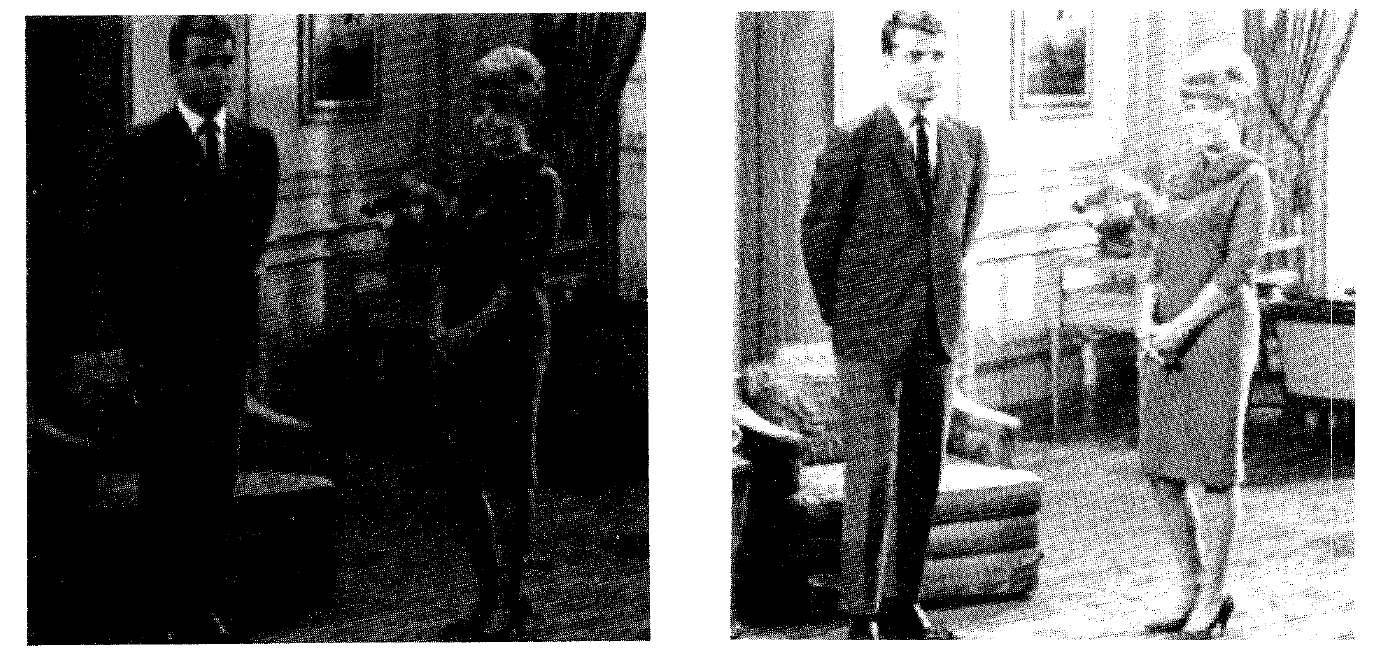
\includegraphics[width=0.45\textwidth]{latex/Couple.png}
    \caption{Image before(left) and after(right) HE algorithm \cite{kim1997contrast}}
    \label{fig:couple}
\end{figure}
the corresponding histogram is shown in Figure \ref{fig:c_his}
\begin{figure}[t]
    \centering
    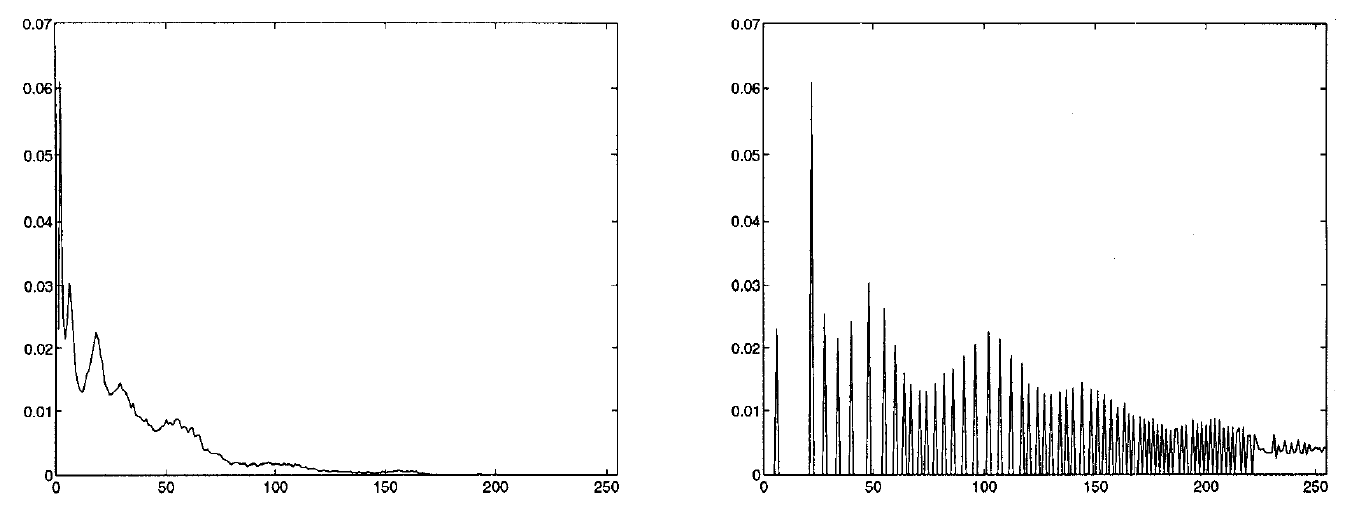
\includegraphics[width=0.45\textwidth]{latex/Couple_histogram.png}
    \caption{Histogram before(left) and after(right) HE algorithm \cite{kim1997contrast}}
    \label{fig:c_his}
\end{figure}

The main idea of Gamma Correction is to enhance the brightness of the image according to the real brightness, as a result, the enhance curve looks like a Gamma Curve, that's why it is called Gamma Correction. And we will talk about \cite{Huang2013Efficient} to explain how basic Gamma Correction works. Simple Gamma Correction equation (also called transform-based gamma correction, TGC) can be written in the following form
\begin{equation}
    T(l)=l_{max}(l/l_{max})^\gamma
\end{equation}
where $l_{max}$ is the maximum intensity of the input,$\gamma$ is called adaptive parameter and $l$ is the intensity of each pixel while $T(l)$ is the intensity after transformation, the curve of different $\gamma$ is shown in Figure \ref{fig:GC}
\begin{figure}
    \centering
    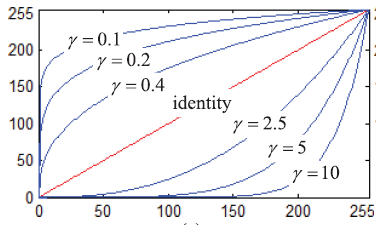
\includegraphics[width=0.45\textwidth]{latex/Gamma_correction.png}
    \caption{Curves of different $\gamma$ \cite{Huang2013Efficient}}
    \label{fig:GC}
\end{figure}
%-------------------------------------------------------------------------
\subsection{Retinex-based Traditional Methods}
Most state-of-art traditional methods are based on Retinex model, which is inspired by \cite{land1977retinex}. The main idea of Retinex-based model can be shown in the function below.
\begin{equation}
    \mathbf{I = R \circ L} 
\end{equation}
where $\textbf{I}$ represents the image observed, and $\textbf{R}$ represents the reflectance of the image while $\textbf{L}$ represents the real illumination of the image and $\circ$ means pixel-wise multiplication. So the function reminds us that an image can be decomposed into two different components and when we do image enhancement, we can utilize them separately. A trick to speed up computation is to do logarithmic transformations on both sides of the equation, for we can convert multiplication to addition in that way.

Here we talk about \cite{LiStructure}, a robust Retinex model to enhance low-light image. In fact, even the state-of-art methods have to admit that denoise is a problem very hard to deal with and noise in image often makes an algorithm perform badly. So in this paper, a robust Retinex model is proposed to deal with the noise in low-light image.

To take noise into consideration, the Retinex function should be changed to 
\begin{equation}
    \mathbf{I = R \circ L + N} \label{con:RobustRetinex}
\end{equation}
where N is the noise component. And it is the noise component that causes the direct logarithmic method fail. In order to solve this equation, the following algorithm is proposed.

First, if we enhance the brightness of the image in the RGB domain, the image must follow gray world hypothesis. And if an image violates it,  enhancing algorithm will lead to color distortion, which shouldn't be allowed. So we transform the image from RGB domain to HSV domain and apply the algorithm on the V component only. Here we treat V component of the image as the left side of Equation \ref{con:RobustRetinex}.

The decomposition algorithm to get $\textbf{R}$ and $\textbf{L}$ of the original image is as follows:
\begin{equation}
    \mathop{\arg\min}\limits_{\mathbf{R,L}}\mathbf{ \left\|R \circ L - I \right\|}_F^2+\beta \mathbf{ \left\| \nabla L\right\|}_1 + \omega \mathbf{\left\| \nabla R - G \right\|}_F^2
\end{equation}
here $\beta$ and $\omega$ are coefficients that control the weight of three parts of the objective function. The first part of the objective function constrains the fidelity between the observed image $\mathbf{I}$ and the recomposed $ \mathbf{R \circ L}$. The second part corresponds to the total variation sparsity and the smoothness of the illumination map  $\mathbf{L}$. The last part has a parameter G, which is modified from $\mathbf{\nabla I}$, and its definition is shown in Equation \ref{con:defG},\ref{con:defK}. This part is used to control the structural similarity and improve the structural similarity between the enhanced image and the original image.
\begin{align}
    &\mathbf{G = K \circ \nabla I} \label{con:defG}\\
    &\mathbf{K} = 1 + \lambda e^{-|\nabla \mathbf{I}|/\sigma} \label{con:defK}
\end{align}
here $\lambda $ controls the degree of the amplification and $\sigma$ controls the amplification rate of different gradients. In this paper, both of them are set to 10.

Based on the method above, a further approach is to explicitly estimate the noise map, and we just have to modify the equations above a little like this:
\begin{equation}
\begin{split}
    \mathop{\arg\min}\limits_{\mathbf{R,L,N}}\mathbf{ \left\|R \circ L + N - I \right\|}_F^2+\beta \mathbf{ \left\| \nabla L\right\|}_1 \\
    + \omega \mathbf{\left\| \nabla R - G \right\|}_F^2 + \delta \mathbf{ \left\| \nabla N\right\|}_F^2 \label{con:longeq}
\end{split}
\end{equation}
where $\mathbf{N}$ is the estimated noise map, $ \mathbf{ \left\| \nabla N\right\|}_F^2$ constrains the overall intensity of the noise. And the modification of $\mathbf{G}$ is like this:
\begin{align}
    &\mathbf{G = K \circ \nabla \hat{I}} \\
    &\mathbf{K} = 1 + \lambda e^{-|\nabla \mathbf{\hat{I}}|/\sigma}
\end{align}
where
\begin{equation}
    \mathbf{\hat{I}} = \begin{cases}
    0 , &if |\nabla \mathbf{I}|< \varepsilon, \\
    \nabla \mathbf{I} , &otherwise.
    \end{cases}
\end{equation}

The solution to the objective function \ref{con:longeq} is calculated by  alternating direction minimization technique (ADM). To simplify the objective function, we replace $\mathbf{\nabla L}$ with a new variable $\mathbf{T}$, then we get
\begin{equation}
\begin{split}
    \mathop{\arg\min}\limits_{\mathbf{R,L,N}}&\mathbf{ \left\|R \circ L + N - I \right\|}_F^2+\beta \mathbf{ \left\|T\right\|}_1 + \omega \mathbf{\left\| \nabla R - G \right\|}_F^2 \\
    &+ \delta \mathbf{ \left\| \nabla N\right\|}_F^2,  s.t. \mathbf{ T = \nabla{L}}. \label{con:fin_arg}
\end{split}
\end{equation}    
then introduce Lagrange multiplier $\mathbf{Z}$, get the Lagrangian function
\begin{equation}
\begin{split}
    \mathcal{L}(\mathbf{R,L,N,T,Z}) = &\mathop{\arg\min}\limits_{\mathbf{R,L,N}}\mathbf{ \left\|R \circ L + N - I \right\|}_F^2 \\
    &+\beta \mathbf{ \left\|T\right\|}_1 + \omega \mathbf{\left\| \nabla R - G \right\|}_F^2 \\
    &+ \delta \mathbf{ \left\| \nabla N\right\|}_F^2 + \Phi(\mathbf{Z, \nabla L - T}) \label{con:fin}
\end{split}
\end{equation}    
where $\Phi(\mathbf{A,B}) = \langle \mathbf{A, B} \rangle + \frac{\mu}{2}\mathbf{ \left\|B\right\|}_F^2$, $\langle \cdot,\cdot \rangle$ represents matrix inner product, $\mu$ is a positive scalar.

Equation \ref{con:fin} can be solved by alternately iterating and optimizing the variables $\mathbf{R,L,N,T,Z}$ and $\mu$. Pseudo code is shown by Algorithm \ref{alg}, and please refer to \cite{LiStructure} for the details of the iterating method. 

\begin{algorithm}[t]
\caption{Solution to problem \ref{con:fin_arg}} \label{alg}
\hspace*{0.02in} {\bf Input:} 
The input image $\mathbf{I}$, the adjusted gradient $\mathbf{G}$.\\
\hspace*{0.02in} {\bf Initialization:}
$\mathbf{L}^{(0)} = \mathbf{I}$, $\mathbf{N^{(0)} = Z^{(0)} = T^{(0)} = 0}$, $k = 0$, $\mu^{(0)} = 1$, $\rho = 1.5$ \\
\hspace*{0.02in} {\bf Output:} 
$\mathbf{R^{(k)}, L^{(k)}, N^{(k)}}.$ 
\begin{algorithmic}[1]
\While{$ not\,converged$}
    \State Update $\mathbf{R^{(k+1)}}$
    \State Update $\mathbf{L^{(k+1)}}$
    \State Update $\mathbf{N^{(k+1)}}$
    \State Update $\mathbf{T^{(k+1)}}$
    \State Update $\mathbf{Z^{(k+1)}}$ and $\mu^{(k+1)}$
    \State $k = k + 1$
\EndWhile
\end{algorithmic}
\end{algorithm}

At last, a simple gamma correction will be applied to make our result more accurate
\begin{align}
    &\mathbf{\hat{I} = R \circ \hat{L}},\\
    &\mathbf{\hat{L} = L^{\frac{1}{\gamma}}}
\end{align}

Researchers from the same group are not limited to traditional methods though they focus on Retinex-based low-light image enhancement. They also investigated on deep-learning methods to solve the problem, such as \cite{wang2018gladnet} and \cite{Wei2018Deep}. Both of them constructed the network according to Retinex theory and the second one can be regarded as the follow-up work of the first one, for the network proposed in the first paper acts as a part of that in the second one. Here we will talk about the second one\cite{Wei2018Deep}, which proposed a network called  Retinex-Net.

The Retinex-Net is composed of two sub-nets, one is Decom-Net, which is used for decomposition the image \textbf{S} into reflectance \textbf{R} and illumination \textbf{I}, the other is called Enhance-Net, which is used for illumination adjustment. The framework of Retinex-Net is shown in Figure \ref{fig:Retinex-Net}, the Retinex equation here has the following form:
\begin{equation}
    \mathbf{S = R \circ I} 
\end{equation}
\begin{figure}[t]
    \centering
    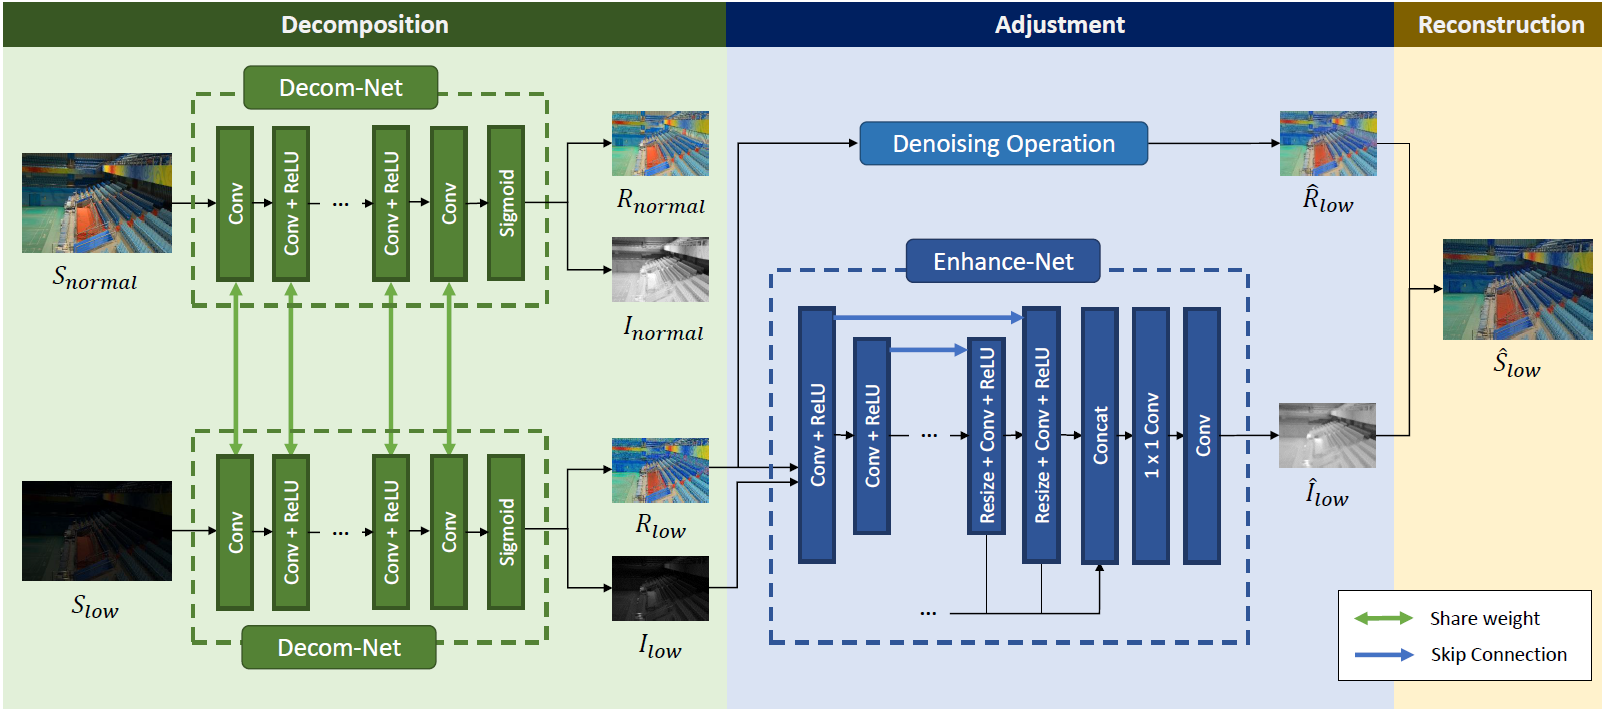
\includegraphics[width=0.45\textwidth]{latex/Retinex Net.png}
    \caption{Framework of Retinex-Net \cite{Wei2018Deep}}
    \label{fig:Retinex-Net}
\end{figure}

As shown in Figure \ref{fig:Retinex-Net}, Decom-Net takes low-light image $S_{low}$ and normal-light image $S_{normal}$ as input, then respectively estimate $ I_{low}$ and $ R_{low}$ for $ S_{low}$ and  $I_{normal}$, $ R_{normal}$ for $ S_{normal}$. To make these estimations, first use a 3 $\times$ 3 convolutional layer to extract features, then several convolutional layers with ReLU as activation function are used to map the RGB image to reflectance and illumination component, at last, a 3 $\times$ 3 convolutional layer is used to construct $R$ and $I$ from feature space, the sigmoid function after this layer is used to constrain them into range [0, 1].

The loss function of Decom-Net, $\mathcal{L}_{decom}$ is defined below
\begin{equation}
    \mathcal{L}_{decom} = \mathcal{L}_{recon} + \lambda_{ir}\mathcal{L}_{ir} + \lambda_{is}\mathcal{L}_{is}
\end{equation}
where $\lambda_{ir}$ and $\lambda_{is}$ are coefficients to balance the weight of different parts of the loss function, the three parts of $\mathcal{L}_{decom}$ respectively evaluates the similarity between the original image and estimated image, the consistency of reflectance and the structure smoothness, their definitions are show below
\begin{align}
    &\mathcal{L}_{recon} = \sum_{i=low, normal}\sum_{j=low, normal}\lambda_{i,j}\left\|R_i \circ I_j - S_j\right\|_1 \\
    &\mathcal{L}_{ir}= \left\|R_{low} - R_{normal}\right\|_1 \\
    &\mathcal{L}_{is}= \sum_{i=low,normal}\left\|\nabla I_i \circ exp(-\lambda_g\nabla R_i)\right\| \label{con:lis}
\end{align}
where $\lambda_g$ in Equation \ref{con:lis} is a coefficient balancing the strength of structure-awareness. 

As for the Enhance-Net, it is an adjusted auto-encoder. The input image is first down-sampled, for a small scale ensures the network can have a perspective of large-scale illumination distribution, after getting the information of illumination distribution, up-sampling block will reconstruct local illumination distribution. The loss function $\mathcal{L}_{enhance}$ is shown below
\begin{equation}
    \mathcal{L}_{enhance}=\mathcal{L}_{recon} + \mathcal{L}_{is}
\end{equation}
where
\begin{align}
    &\mathcal{L}_{recon} = \left\|R_{low} \circ \hat{I}- S_{normal}\right\|_1 \\
    &\mathcal{L}_{is}= \sum_{i=low,normal}\left\|\nabla I_i \circ exp(-\lambda_g\nabla R_i)\right\| 
\end{align}

As for the latest progress of Retinex-based traditional methods, we choose two papers published in year 2019 \cite{Xu2019STAR,kurihara2019low}, both of them add their own restrictions to the optimization function. Here we will talk about \cite{Xu2019STAR}.

Structure and Texture Aware Retinex (STAR) model \cite{Xu2019STAR} focus on better structure and texture preservation while enhancing low-light image. It is known that denoise is an important part of dark image enhancement, however, when we apply denoise algorithm, structure and textures of bright region are often mistaken as noise due to high-gradient.

In order to preserve the structure information, the best way is to extract the structural map from the beginning, so the paper choose two typical filters for structure extraction algorithms, i.e. Total Variation(TV) \cite{rudin1992nonlinear} and Mean Local Variance(MLV) \cite{cai2017joint}
TV computes the absolute gradients of an input image as a guidance map:
\begin{equation}
    f_{TV}(\mathbf{O}) = |\nabla \mathbf{O}|
\end{equation}
equation of MLV is shown below:
\begin{equation}
    f_{MLV}(\mathbf{O}) = |\frac{1}{|\Omega|}\sum_\Omega \nabla \mathbf{O}|
\end{equation}

However, the two methods cannot be directly used in low-light image enhancement, since they are prone to capture structural information, a solution to this problem is to add an exponent term to them, so adjusted functions (called ETV and EMLV )are shown below:
\begin{equation}
    f_{ETV}(\mathbf{O}) = |\nabla \mathbf{O}|^\gamma \label{con:etv}
\end{equation}
\begin{equation}
    f_{EMLV}(\mathbf{O}) = |\frac{1}{|\Omega|}\sum_\Omega \nabla \mathbf{O}|^\gamma \label{con:emlv}
\end{equation}
and $\gamma$ can determine the sensitivity to the gradients of $\mathbf{O}$.

In this method, we also solve illumination($\mathbf{I}$) and reflectance($\mathbf{R}$) via iterative algorithm, based on Equation \ref{con:etv},\ref{con:emlv}, we can write ETV based weighting matrix used for the first iteration as follows:
\begin{align}
    &\mathbf{S}_0 = 1 \oslash (|\nabla \mathbf{I}_0|^\gamma_s + \varepsilon) \\
    &\mathbf{T}_0 = 1 \oslash (|\nabla \mathbf{R}_0|^\gamma_t + \varepsilon)
\end{align}
for EMLV:
\begin{align}
    &\mathbf{S}_0 = 1 \oslash (|\frac{1}{|\Omega|}\sum_\Omega \nabla \mathbf{I}_0 |^\gamma_s + \varepsilon) \\
    &\mathbf{T}_0 = 1 \oslash (|\frac{1}{|\Omega|}\sum_\Omega \nabla \mathbf{R}_0 |^\gamma_t + \varepsilon)
\end{align}
where $\gamma_s > 1$ and $\gamma_t < 1$ are two exponential parameters
to adjust the structure and texture awareness for illumination
and reflectance decomposition.
With the definition of the structure extraction function, the optimization function of STAR can be written as follows(like \cite{LiStructure}, there are three components):
\begin{equation}
    \mathop{\arg\min}\limits_\mathbf{I,R} \left\|\mathbf{O - I \odot R}\right\|_F^2 + \alpha \left\|\mathbf{S_0 \odot \nabla I }\right\|_F^2 + \beta \left\|\mathbf{T_0 \odot \nabla R }\right\|_F^2
\end{equation}
Iterative solving method is similar to Algorithm \ref{alg}, for details, refer to \cite{Xu2019STAR}, we will not talk about it here.

\subsection{Illumination Map centered Traditional Methods}
Apart from traditional Retinex-based methods, there are also other traditional methods to enhance low-light images, these methods although based on Retinex theory too, but only focus on part of the decomposed image. The first paper we will talk about proposed a method called LIME \cite{guo2016lime}, which focus on illumination map only instead of utilizing both illumination map and reflection map, reducing the computational cost.

 In LIME, we use $\mathbf{L}$ to represent the original image, and the illumination map is represented by $\mathbf{T}$, so the Retinex equation here has the following form:
 \begin{equation}
    \mathbf{L = R \circ T} \label{con:retinexmodel3}
\end{equation}

 From Equation \ref{con:retinexmodel3}, we can see that if we are very confident of our estimation result, there is no need to estimate both $\mathbf{R}$ and $\mathbf{T}$, for $\mathbf{L}$ is known, one can be calculated from the other. So LIME tries to find a way to get illumination map $\mathbf{T}$ as accurate as possible and calculate $\mathbf{ R = L / T}$ , reducing computational cost.
 
As we know, the illumination is at least the maximal value of three channels at a certain location, so the initial estimation of illumination map can be calculated using the following function:
\begin{equation}
    \mathbf{\hat{T}(x)} \leftarrow \max_{c \in \{ R,G,B\}} \mathbf{L}^c(x) \label{con:initial}
\end{equation}
with this, $\mathbf{R}$ can be calculated:
\begin{equation}
    \mathbf{R}(x) = \mathbf{L}(x)/(\max_c \mathbf{L}^c(x)+ \varepsilon) \label{con:simple}
\end{equation}

It is noticed in \cite{dong2011fast} that inverted low-light image looks like hazy images , and dehaze algorithm also works well on it. Based on this theory, we can get another equation of calculating $\mathbf{R}$ :
\begin{equation}
    \mathbf{R}(x) = \frac{\mathbf{L}(x) -1 + a }{1- \frac{1}{a} + \max_c \frac{\mathbf{L}^c(x)}{a} + \varepsilon } + (1-a). \label{con:complex}
\end{equation}
we can see when $a = 1 $ Equation\ref{con:simple} and Equation\ref{con:complex} are the same, but when $a \not = 1$, they are no longer the same. And the latter one doesn't perform better than former one. Besides, the former one is simple to achieve, so we choose to use Equation\ref{con:simple} .

Based on Equation\ref{con:initial}, to preserve the overall structure and smooth the textural details, we define a new way to calculate $\mathbf{T}$ as shown below:
\begin{equation}
    \min_{\mathbf{T}}\left\|\mathbf{\hat{T} - T}\right\|_F^2 + \alpha \left\|\mathbf{W \circ \nabla T}\right\|_1 \label{con:targetT}
\end{equation}
where $\alpha$ is the balance coefficient, $\left\|\mathbf{ \cdot }\right\|_F$ means Frobenious norm and $\mathbf{W}$ is a weighting matrix, to define $\mathbf{W}$, first we decompose $\mathbf{W}$ into horizontal and vertical component:
\begin{equation}
    \lim_{\varepsilon \rightarrow 0^+}\sum_x \sum_{d \in \{h,v\}}\frac{\mathbf{W}_d(x)(\nabla_d \mathbf{T}(x))^2}{|\nabla_d \mathbf{T}(x)| + \varepsilon} = \left\|\mathbf{W \circ \nabla T }\right\|_1  \label{con:Wdec}
\end{equation}
with Equation\ref{con:Wdec}, Equation\ref{con:targetT} can be transformed to
\begin{equation}
     \min_{\mathbf{T}}\left\|\mathbf{\hat{T} - T}\right\|_F^2 + \alpha \sum_x \sum_{d \in \{h,v\}}\frac{\mathbf{W}_d(x)(\nabla_d \mathbf{T}(x))^2}{|\nabla_d \mathbf{T}(x)| + \varepsilon}
\end{equation}
 
As for the choice for $\mathbf{W}_h$ and $\mathbf{W}_v$, there are three categories, each of them has their own effects \\
$Strategy \uppercase\expandafter{\romannumeral1}$:
\begin{equation}
    \mathbf{W}_h(x) \leftarrow 1; \mathbf{W}_v(x) \leftarrow 1
\end{equation}
$Strategy \uppercase\expandafter{\romannumeral2}$:
\begin{equation}
    \mathbf{W}_h(x) \leftarrow \frac{1}{|\nabla_h\mathbf{\hat{T}(x)}|+ \varepsilon}; \mathbf{W}_v(x) \leftarrow \frac{1}{|\nabla_v\mathbf{\hat{T}(x)}|+ \varepsilon}
\end{equation}
$Strategy \uppercase\expandafter{\romannumeral3}$:
\begin{align}
    &\mathbf{W}_h(x) \leftarrow \sum_{y \in \Omega(x)}\frac{G_\sigma(x,y)}{|\sum_{y \in \Omega(x)} G_\sigma(x,y)\nabla_h(\hat{\mathbf{T}}(y))|+\varepsilon}; \\
    &\mathbf{W}_v(x) \leftarrow \sum_{y \in \Omega(x)}\frac{G_\sigma(x,y)}{|\sum_{y \in \Omega(x)} G_\sigma(x,y)\nabla_v(\hat{\mathbf{T}}(y))|+\varepsilon}
\end{align}
where $G_\sigma(x,y)$ is a Gaussian function:
\begin{equation}
    G_\sigma(x,y) \propto exp(- \frac{dist(x,y)}{2\sigma^2})
\end{equation}

The solving method also first transform into Lagrange format, then utilize it iteratively, we won't waste time talking about it again here, for detailed solving method, please refer to\cite{guo2016lime}.

The follow-up works of LIME mainly focus on enhancing low-light image with deep-learning method, including \cite{zhang2019kindling,wang2019underexposed}, there are also papers propose other form of $ \mathbf{T}$, such as \cite{hao2018low}, here we talk about the two deep-learning methods.

 The same research group proposed a deep-learning method for low-light image enhancement\cite{zhang2019kindling} in 2019. This deep-learning method is based on Retinex-model, i.e. an image is decomposed into illumination and reflectance components. The learning method is very interesting, for it doesn't rely on ground truth, only requires the two images are taken in the same scene and the exposure are different. And as the scene of the two images are the same, their reflectance map will be the same, so we can take advantage of it. Not relying on ground truth is of great importance, for the ground truth data is hard to get, resulting in lack of datasets of low-light image enhancement. The framework of the network is shown in Figure \ref{fig:kindle}
\begin{figure}[t]
    \centering
    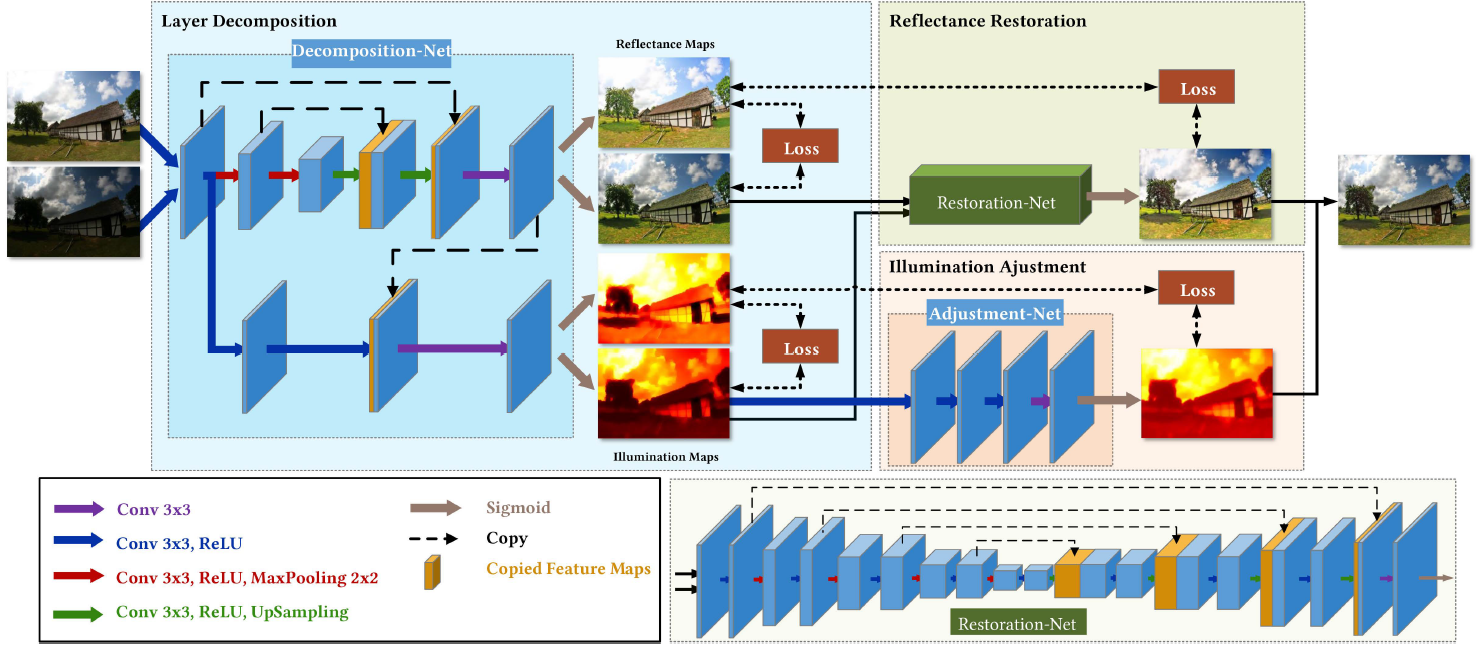
\includegraphics[width=0.45\textwidth]{latex/Kindle.png}
    \caption{KinD network architecture \cite{zhang2019kindling}}
    \label{fig:kindle}
\end{figure}

The whole network contains three parts: Layer Decomposition, Reflectance Restoration, Illumination Adjustment. Each of them corresponds to a sub-net: Decomposition-Net for Decomposition, Restoration-Net for Reflectance Restoration and Adjustment-Net for Illumination Adjustment, we will introduce these sub-nets below. \\
\textbf{Decomposition Net} \\
The decomposition network works on reflectance and illumination parallelly,
reflectance branch first use a 5-layer U-Net, then a convolutional layer and at last a Sigmoid layer. The illumination branch is composed of two conv+ReLU layers and a conv layer on concatenated feature maps from the reflectance branch (for possibly excluding textures from the illumination), finally pass a Sigmoid layer.
Loss function is shown below:
\begin{equation}
    \mathcal{L}^{LD} = \mathcal{L}^{LD}_{rec}+\alpha \mathcal{L}^{LD}_{rs}+\beta \mathcal{L}^{LD}_{is}+ \gamma \mathcal{L}^{LD}_{mc}
\end{equation}
where $LD$ is short for Layer Decomposition, $\alpha$,$\beta$,$\gamma$ are all coefficients, here we take $\alpha = 0.01$, $\beta = 0.15$, $\gamma = 0.2 $. The four sub losses are defined as below:
As we will always put in a pair of images $[\mathbf{I}_l, \mathbf{I}_h]$, as Figure\ref{fig:kindle} shows, we will get two pairs of map, i.e. $[\mathbf{R}_l,\mathbf{R}_h]$ and $[\mathbf{L}_l,\mathbf{L}_h]$. The restriction on the former one should be $\mathbf{R}_l$ and $\mathbf{R}_h$  are as similar as possible, so we define $\mathcal{L}_{rs}^{LD}$ as
\begin{equation}
    \mathcal{L}_{rs}^{LD} = \left\|\mathbf{R}_l - \mathbf{R}_h\right\|_1
\end{equation}

As for $[\mathbf{L}_l,\mathbf{L}_h]$, our constriction is that they should be piece-wise smooth and mutually consistent, the former can be defined as follows:
\begin{equation}
    \mathcal{L}_{is}^{LD} = \left\| \frac{\nabla \mathbf{L}_l}{\max(|\nabla \mathbf{I}_l|, \varepsilon)}\right\|_1 + \left\| \frac{\nabla \mathbf{L}_h}{\max(|\nabla \mathbf{I}_h|, \varepsilon)}\right\|_1
\end{equation}
and mutually consistent can be restricted by 
\begin{align}
   &\mathcal{L}_{mc}^{LD} = \left\|\mathbf{M} \circ exp(-c \cdot \mathbf{M})\right\|_1 \\
   & \mathbf{M = |\nabla L_l| + |\nabla L_h|}
\end{align}

At last, we should of course take reconstruction error into account, so
\begin{equation}
    \mathcal{L}_{rec}^{LD} = \left\| \mathbf{I_l - R_l \circ L_l} \right\|_1 + \left\| \mathbf{I_h - R_h \circ L_h} \right\|_1
\end{equation}
\textbf{Reflectance Restoration Net}\\
As there is no ground truth, we must choose either $\mathbf{R_l}$ or $\mathbf{R_h}$ as ground truth if we want to add a restriction to estimated reflectance $\mathbf{\hat{R}}$. So for the Reflectance Restoration Net, the loss function should be written like below:
\begin{equation}
    \mathcal{L}^{RR} = \left\| \mathbf{\hat{R} - R_h } \right\|_2^2  - SSIM(\mathbf{\hat{R},R_h}) + \left\| \mathbf{\nabla \hat{R} - \nabla R_h } \right\|_2^2
\end{equation}
where $SSIM(\cdot,\cdot)$ is the structural similarity measurement, the third part of the loss function concentrates on texture and structure.\\
\textbf{Illumination Adjustment Net} \\
When we turn to illumination map, we also face the problem that there is no ground truth for illumination map. To deal with this, we roughly calculate the ratio of strength $\alpha$ for paired illumination maps to give a description of illumination and use it to transform between different illumination maps. The definition of $\alpha$ is the mean of $\mathbf{L}_t/\mathbf{L}_s$ (the division is element-wise). For example. when $\alpha > 1$, it means adjusting a dark image to a bright image, otherwise, adjust a bright one to a dark one. When we really use the network, $\alpha$ is set in advance by users. The loss function is shown below:
\begin{equation}
    \mathcal{L}^{IA} = \left\| \mathbf{\hat{L}} - \mathbf{L}_t\right\|_2^2 + \left\| \mathbf{|\nabla \hat{L}| - |\nabla L_t |}\right\|_2^2
\end{equation}
where $\mathbf{L_t}$ can be $\mathbf{L_h}$ or $\mathbf{L_l}$. When compared to gamma correction, we found network trained with this loss function can increase more light on bright region and less on dark region, which shows this method is better than gamma correction.

Another deep-learning method proposed in 2019\cite{wang2019underexposed} inherited the main idea of \cite{guo2016lime},i.e. if our estimation of illumination map is good enough, we can easily calculate reflectance map from the original image and illumination map. In fact, in this method, the illumination map is regarded as a mapping function and the reflectance is regarded as independent variable.  Here our decomposition is shown below:
\begin{equation}
    I = S \ast \tilde{I}
\end{equation}
network architecture is shown in Figure \ref{fig:Under-Net}.
\begin{figure}[t]
    \centering
    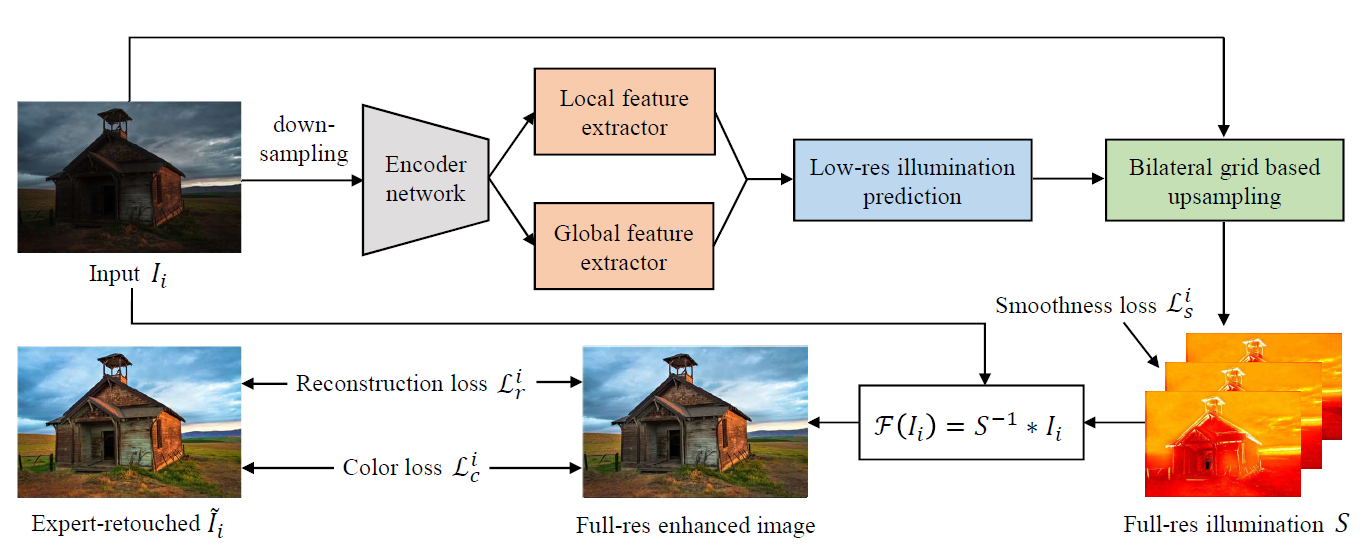
\includegraphics[width=0.45\textwidth]{latex/Under_net.png}
    \caption{Network architecture \cite{wang2019underexposed}}
    \label{fig:Under-Net}
\end{figure}
From Figure \ref{fig:Under-Net} we can see the whole pipeline: First for an input image, down-sample to ensure the whole algorithm run on low-resolution image, which will decrease computational cost. Then extract both local and global feature with an encoder network, the local features include contrast, detail sharpness, shadow, and highlight; the global features include color distribution, average brightness, and scene category. With all these features taken into consideration, the estimated illumination map will preserve more structural information and will be more accurate. After that, we mix them up and up-sample to get a high-resolution illumination map, then add a smoothness restriction. At last, we calculate the reflection component(also the enhanced result).

The network works by learning the illumination mapping from a set of N image pairs $\{(I_i, \tilde{I}_i)\}_{i=1}^N$, where $\tilde{I}_i$ is the ground truth, and the loss function for this network has three parts, it is shown below:
\begin{equation}
    \mathcal{L}= \sum_{i=1}^N \omega_r\mathcal{L}_r^i + \omega_s\mathcal{L}_s^i + \omega_c\mathcal{L}_c^i
\end{equation}
where $\omega_r$, $\omega_s$, $\omega_c$ are corresponding weights, empirically, we set them to 1, 2, 1 respectively. $\mathcal{L}_r^i$, $\mathcal{L}_s^i$, $\mathcal{L}_c^i$ represents reconstruction loss, smoothness loss and color loss, their definition are shown below:\\
\textbf{Reconstruction Loss}
\begin{equation}
    \begin{split}
        \mathcal{L}_r^i & = \left\|I_i - S \ast \tilde{I}_i\right\|^2,\\
       & s.t. (I_i)_c \leq (S)_c \leq 1, \forall\,pixel\,channel\,c
    \end{split}
\end{equation}
where $()_{c \in \{r,g,b\}}$ \\
\textbf{Smoothness Loss}
\begin{equation}
    \mathcal{L}_s^i = \sum_p \sum_c \omega_{x,c}^p(\partial_x S_p)_c^2 + \omega_{y,c}^p(\partial_y S_p)_c^2 
\end{equation}
where
\begin{equation}
    \begin{split}
        \omega_{x,c}^p = (|\partial_x L_i^p|_c^\theta + \varepsilon)^{-1} \\
        \omega_{y,c}^p = (|\partial_y L_i^p|_c^\theta + \varepsilon)^{-1}
    \end{split}
\end{equation}
here, $L_i$ is the logarithmic image of input image $I_i$, $\theta$ is a parameter controls the sensitivity to gradients, which is set to 1.2, $\varepsilon$ is used to prevent division by zero. \\
\textbf{Color Loss} \\
First we represent the enhanced image with mark $\hat{I} $
\begin{equation}
    \mathcal{L}_c^i = \sum_p \angle((\hat{I}_i)_p,(\tilde{I}_i)_p)
\end{equation}
where $()_p$ denotes calculate pixel by pixel, $\angle(,)$ calculates the angle between two vectors, this means we regard the R,G,B channel of a pixel as a 3D vector. The reason why we choose angular error instead of L2 norm error is that L2 norm can't reflect whether the vectors have the same direction, which is more important when considering color only.

\subsection{CNN-based Deep Learning Methods}
Since researchers started to apply deep learning methods on low-light image enhancement, many different types of networks have been proposed, here we choose some representative papers using Convolutional Neural Network (CNN) and AutoEncoder methods to talk about, in this section, we will talk about CNN-based deep learning methods and in the next section, AutoEncoder methods. 

The first paper to talk about is\cite{chen2018learning}, which proposed a fully-convolutional network (FCN) to learn a new pipeline for extremely low-light image. The perspective of this article is very interesting. It points out that most of the state-of-art methods are based on the prior that the low-light condition is not so bad that existing image processing pipeline fails. And when the light condition is very bad, we need a new pipeline to deal with RAW images to produce enhanced image instead of using a bad pipeline first, then adjust the image produced by it.

\begin{figure}[t]
    \centering
    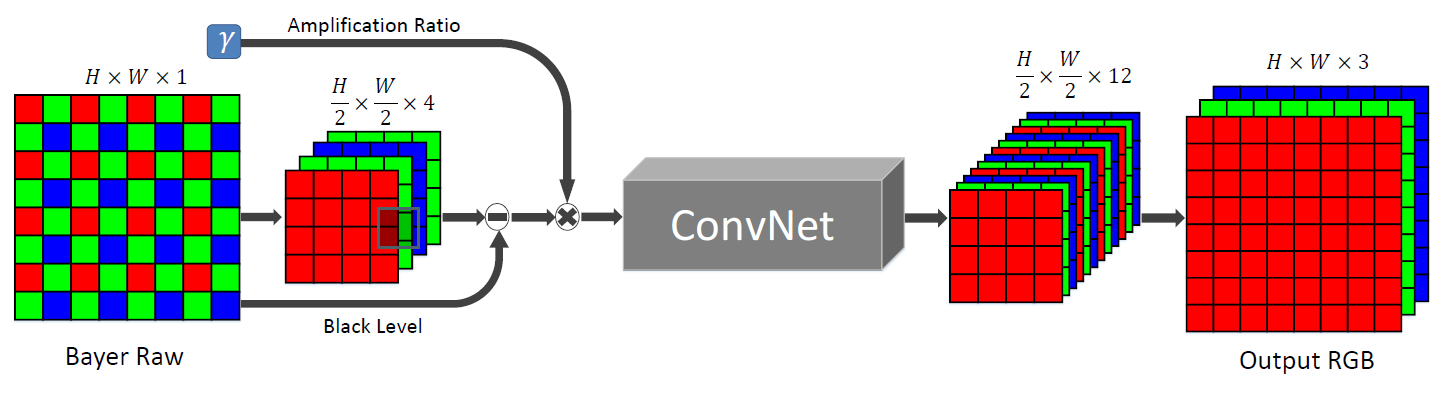
\includegraphics[width=0.45\textwidth]{latex/new_pipeline.png}
    \caption{Network architecture \cite{chen2018learning}}
    \label{fig:newPipeline}
\end{figure}
The network framework is shown in Figure\ref{fig:newPipeline}. Note that our network is used for producing a new image processing pipeline, so the input is RAW data. For Bayer form RAW data, first decompose the data into four channels and the resolution decrease to half of the original data. If the RAW data's form is X-Trans, we will pack it into nine channels. After adding in an amplification ratio $\gamma$, our packed data will be sent into a fully-convolutional network (FCN), the reason why we choose FCN is that many previous experiments have shown that FCN can realize many parts of the image processing pipeline, so it is natural to think that FCN can fulfill the whole image processing pipeline. After the FCN, we get a twelve channel image with half resolution, so we just have to recover it to original resolution, then we will get the result.

As for the loss function, there is nothing special, just choose $L1$ loss and use Adam optimizer to optimize it. In fact, the most interesting part is the thought that we can use network to learn a new image processing pipeline specially for low-light images.

\subsection{AutoEncoder-based Deep Learning Methods}
Apart from CNN method, AutoEncoder is also a popular choice for deep-learning methods, here we will first talk about \cite{lore2017llnet}, which is a famous article in low-light image enhancement, and has inspired many later researches, though the paper has been published for a long time, it is still well-worth reading.

Since LLNet is among the first papers of using deep-learning methods to solve low-light image enhancement, the network framework isn't very complex. Researchers proposed two types of framework, one is simultaneously learn resolution enhancing and de-noising, the other is to learn them separately, which is called Separated LLNet(S-LLNet). Their frameworks are shown in Figure \ref{fig:llnet}
\begin{figure}[t]
    \centering
    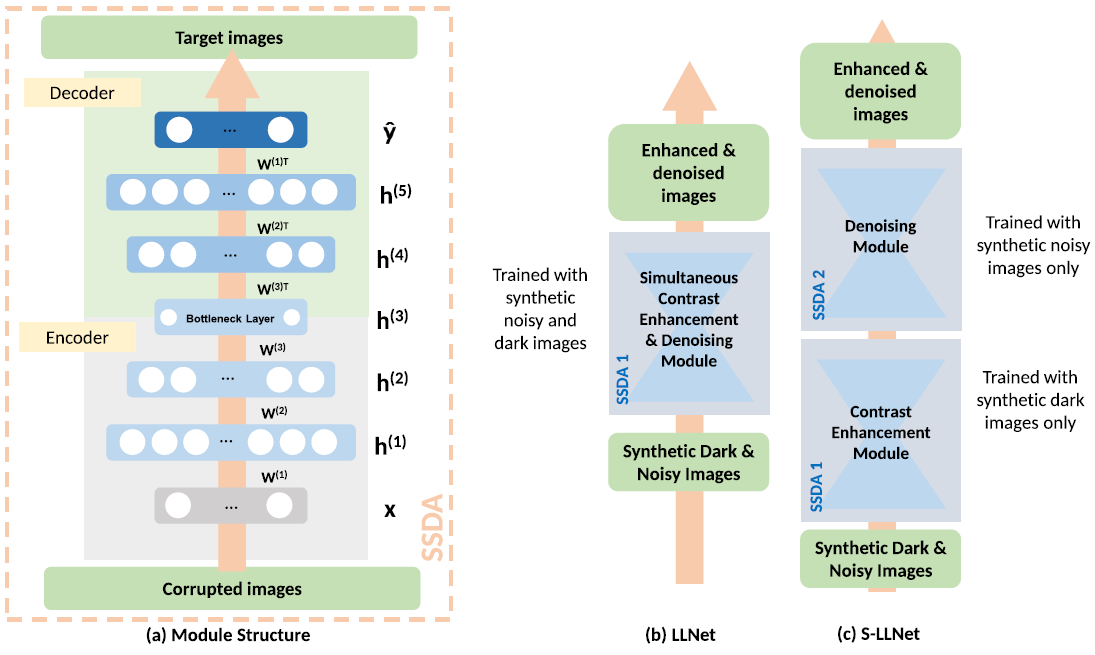
\includegraphics[width=0.45\textwidth]{latex/llnet.png}
    \caption{Network architecture \cite{lore2017llnet}}
    \label{fig:llnet}
\end{figure} 

To be precise, the net should be called Stacked Sparse Denoising
Autoencoder(SSDA), which is composed of many Denoise Autoencoders(DA), the loss function of each DA is shown below:
\begin{equation}
    \begin{split}
        \mathcal{L}_{DA}(\mathcal{D};\theta) = & \frac{1}{N}\sum_{i = 1}^N \frac{1}{2} \left\|y_i - \hat{y}(x_i)\right\|_2^2 + \beta \sum_{j=1}^K KL(\hat{\rho_j} || \rho) \\
        & +\frac{\lambda}{2}(\left\|W \right\|_F^2 + \left\|W' \right\|_F^2)
    \end{split}
\end{equation}
where N is the number of patches, $\theta = \{W, b ,W', b' \}$ are parameters, $\rho$ is target activation and $\hat{\rho}$ is empirical average activation of the $j$th hidden unit.
with the loss function of each DA, the whole loss function of SSDA can be written now:
\begin{equation}
    \mathcal{L}_{SSDA}(\mathcal{D};\theta) =  \frac{1}{N}\sum_{i = 1}^N  \left\|y_i - \hat{y}(x_i)\right\|_2^2 + \frac{\lambda}{L}\sum_{i=1}^{2L}\left\|W^{(l)}\right\|_F^2 
\end{equation}\\
where $L$ is the number of stacked DAs, $W^{(l)}$ is the weight for the $l$th layer in the stacked network.

There is a paper \cite{wang2019image} directly inherited the idea of \cite{lore2017llnet}, and proposed a network called CAENet. The found that when LLNet is applied to three-channel images, there are lost of redundant parameters. So they proposed convolutional autoencoder network(CAENet), which replaced original FCN by a convolutional network, making the training more efficient while getting a better performance.

\section{Discussions}
Methods such as HE or gamma correction can't get a good enough performance because they only consider increasing the contrast, but on the other hand, if we add more denoise restrictions to these algorithms, their performance will be better. What's more, they can be a part of more complex low-light image enhancing methods and as they have much lower computational cost, when resources are very limited, they will be a good choice.

As for Retinex-based traditional methods, they are now the main research aspect of traditional methods and their performance are very good. The main problem these methods are facing is the loss of structural information and how to better denoise the image. In the future, referring to other image enhancing methods, such as dehaze or rain-removal algorithms may be a good choice to acquire new inspiration.

Recently, more and more traditional methods focus on the accuracy of illumination map and proposed many illumination-map centered methods. These methods have the advantage that the computation cost is lower, for estimating two unknown variables from one image is a highly ill-conditioned problem, while in contrast, estimating one variable is much more easier.

As for deep learning based methods, almost all the state-of-art deep-learning methods suffer from lack of training dataset, for the ground truth of an image is hard to define and hard to get. If we manually enhance images as ground truth, the workload will be unbearable. So in the future, finding a good way to define and generate dataset of low-image enhancement is still well-worth investigating, though the problem has been existed since the deep-learning methods are used in low-light image enhancement.

Another way to solve the problem of lacking of ground truth is \cite{zhang2019kindling}, which cleverly avoided this problem, and this paper was recently published, so in the future, more investigations should be carried out on it and maybe it is the key to solve the dataset problem.

The method \cite{chen2018learning} surprised us by thinking from a new aspect, but it is hard to use for most of actual algorithms, for RAW data is usually hard to get. Unless we can get RAW data easily one day, this method is hard to popularize.
\section{Conclusion}
In this paper, we had a review on the investigation history of low-light image enhancement, we talked about HE and gamma correction, Retinex-based traditional methods, recently popular illumination-map centered methods and popular deep-learning methods on low-light image enhancement. And we also gave their follow-up work to make the trail of investigation clearer. At last, we discussed the advantages and disadvantages of different methods and pointed out the directions well-worth investigating.

{\small
\bibliographystyle{ieee_fullname}
\bibliography{egbib}
}

\end{document}
